%!TEX root = ../main.tex 

\section{Quels sont les types de régulateurs?}

\begin{frame}{Régulateurs Linéaires vs Switching}
\renewcommand{\arraystretch}{1.4}
\begin{table}
    \centering
    \begin{tabular}{>{\color{UDSgreenSolidarite}}c c | c | c}
        \rowcolor{UDSgreenSolidarite}
        \color{white}\textbf{\faList} & \color{white}\textbf{Critère} & 
        \color{white}\textbf{Régulateur Linéaire} & 
        \color{white}\textbf{Régulateur Switching} \\
        \faDollarSign\ & \textbf{Coût}       
            & {\color{UDSgreenFierte}Faible \cmark} 
            & {\color{red}Moyen à Élevé \xmark} \\
        \faPuzzlePiece\ & \textbf{Complexité} 
            & {\color{UDSgreenFierte}Faible \cmark} 
            & {\color{red}Moyen à Élevé \xmark} \\
        \faPercent\ & \textbf{Efficacité} 
            & {\color{red}Faible \xmark} 
            & {\color{UDSgreenFierte}Très Efficace \cmark} \\
        \faWaveSquare\ & \textbf{Bruit}      
            & {\color{UDSgreenFierte}Faible \cmark} 
            & {\color{red}Moyen à Élevé \xmark} \\
        \faRandom\ & \textbf{\boldmath$V_{out}$} 
            & {\color{red}$V_{out} < V_{in}$ \xmark} 
            & {\color{UDSgreenFierte}$V_{out} \subseteq \mathbb{R}$ \cmark} \\
        \faBolt\ & \textbf{Courant}            
            & {\color{red}Faible à Moyen \xmark}
            & {\color{UDSgreenFierte}Moyen à Élevé \cmark} \\
        \faThermometerHalf\ & \textbf{Température}        
            & {\color{red}Élevée \xmark}            
            & {\color{UDSgreenFierte}Faible à Moyenne \cmark} \\
    \end{tabular}
\end{table}
\end{frame}

\subsection{Régulateurs Linéaires}

\begin{frame}{Régulateur Linéaire (LDO) - Résumé}
    \begin{columns}
        \begin{column}{0.5\textwidth}
            \vspace{-24pt}
            \begin{itemize}
                \item<1-> Régulateur très simple
                \begin{itemize}
                    \item<1-> IC
                    \item<1-> Pièces autours
                \end{itemize}
                \item<2-> Output très stable
                \begin{itemize}
                    \item<2-> PSRR
                \end{itemize}
                \item<3-> $V_{in} > V_{out} > \SI{0.5}{\volt}$
                \item<4-> Très peu efficace
                \begin{itemize}
                    \setlength{\itemsep}{4pt}
                    \item<4-> $I_{in} = I_{out}$
                    \item<4-> $eff = \dfrac{P_{out}}{P_{in}} = \dfrac{V_{out}}{V_{in}}$
                \end{itemize}
                \item<5-> Power dissipée en chaleur!
                \item<5-> Limite le courant
            \end{itemize}
        \end{column}

        \begin{column}{0.5\textwidth}
            \renewcommand{\arraystretch}{1.4}
            \begin{table}
            \centering
            \begin{tabular}{>{\color{UDSgreenSolidarite}}c | c}
                \rowcolor{UDSgreenSolidarite}
                \color{white}\textbf{\faList} & \color{white}\textbf{Régulateur Linéaire}\\
                \faDollarSign\ & {\color{UDSgreenFierte}Faible \cmark}\\
                \faPuzzlePiece\ & {\color{UDSgreenFierte}Faible \cmark}\\
                \ifnum\slideno>1
                \faWaveSquare\ & {\color{UDSgreenFierte}Faible \cmark}\\
                \ifnum\slideno>2 
                \faRandom\ & {\color{red}$V_{out} < V_{in}$ \xmark}\\
                \ifnum\slideno>3 
                \faPercent\ & {\color{red}Faible \xmark}\\
                \ifnum\slideno>4 
                \faThermometerHalf\ & {\color{red}Élevée \xmark}\\
                \faBolt\ & {\color{red}Faible à Moyen \xmark}\\
                \fi\fi\fi\fi
            \end{tabular}
            \end{table}
            \vfill
            \begin{figure}
                \centering
                \includegraphics<-3>[width=0.33\textwidth]{pictures/linear-regulator-7805.png}
            \end{figure}
        \end{column}
    \end{columns}
\end{frame}

\begin{frame}{Régulateur Linéaire - Fonctionnement}
    \begin{figure}
        \centering
        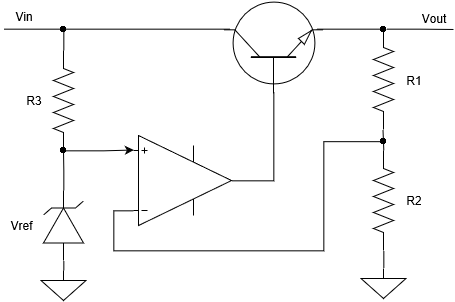
\includegraphics[width=0.9\textwidth]{pictures/linear-regulator.png}
    \end{figure}
\end{frame}

\begin{frame}{Power Supply Ripple Reduction}
    \begin{columns}
        \begin{column}{0.4\textwidth}
            \begin{center}
                $PSRR = \dfrac{\Delta V_{in}}{\Delta V_{out}}$
            \end{center}
        \end{column}
        \pause
        \begin{column}{0.5\textwidth}
            \begin{center}
                $PSRR (dB) = -20 \log \left(\dfrac{\Delta V_{in}}{\Delta V_{out}}\right)$
            \end{center}
        \end{column}
    \end{columns}
    \vfill
    \begin{columns}
        \begin{column}{0.3\textwidth}
            \begin{itemize}
                \item Réduction du bruit
                \item À une fréquence
            \end{itemize}
            \pause
            \vspace{12pt}
            \begin{itemize}
                \item Graphique PSRR
                \item Dépend du courant
            \end{itemize}
        \end{column}
        \begin{column}{0.66\textwidth}
            \begin{figure}
                \centering
                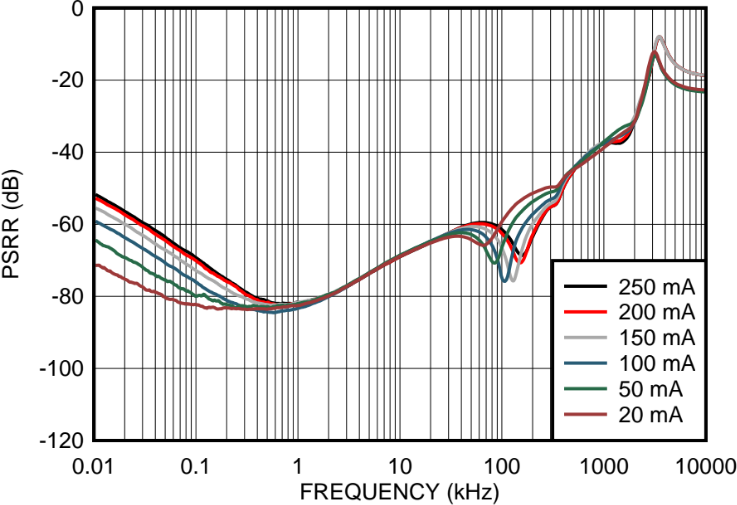
\includegraphics[width=\textwidth]{pictures/psrr-graph.png}
            \end{figure}
        \end{column}
    \end{columns}
\end{frame}

\begin{frame}{Quand choisir un régulateur linéaire?}
\Large
\begin{itemize}
    \item \color{UDSgreenFierte}\faDollarSign \color{black} ~Low-Cost
    \item \color{UDSgreenFierte}\faBolt \color{black} ~Peu de courant
    \item \color{UDSgreenFierte}\faCompress \color{black} ~Peu d'espace
    \item \color{UDSgreenFierte}\faWaveSquare \color{black} ~Bruit très important
    \item \color{UDSgreenFierte}\faPercent \color{black} ~Efficacité peu importante
    \bigskip
    \item \color{UDSgreenFierte}\faLightbulb \color{black} ~À utiliser avec des régulateurs switching!
\end{itemize}

\end{frame}

\subsection{Régulateurs \textit{Switching}}